% Preamble
\documentclass[12pt, twoside]{book}
\usepackage[utf8]{inputenc}
\usepackage{graphicx}
\usepackage{amsmath}
\usepackage{amsfonts}
\usepackage{nicematrix}
\usepackage{algorithm}
\usepackage{algpseudocode}
\usepackage{mathtools} % dcases
\usepackage{multicol}
\usepackage{tcolorbox}
\usepackage{datetime}
\usepackage{caption}
\usepackage{etoolbox}
\usepackage{subfig}
\usepackage{algcompatible}
\usepackage{algpseudocode}
\usepackage{setspace}
\usepackage[a4paper,left=40mm,right=20mm,top=20mm,bottom=20mm,bindingoffset=0mm]{geometry}
\usepackage{fancyhdr}
\usepackage{listings}
\usepackage{color}
\usepackage{hyperref}
\usepackage{enumitem}
\usepackage{attachfile}
\usepackage[toc, acronym]{glossaries}

% Telugu script
\usepackage{fontspec}
\newfontfamily{\tel}[Script=Telugu]{Mandali}

% Custom colors
\definecolor{deepblue}{rgb}{0,0,0.5}
\definecolor{deepred}{rgb}{0.6,0,0}
\definecolor{deepgreen}{rgb}{0,0.5,0}

% Python style for highlighting

\newtheorem{theorem}{Theorem}[section]
\newtheorem{definition}{Definition}[section]
\newtheorem{notation}{Notation}[section]
\newtheorem{remark}{Remark}[section]
\newtheorem{corollary}{Corollary}[theorem]
\newtheorem{lemma}[theorem]{Lemma}
\newtheorem{problem}[theorem]{Problem}

\newcommand{\twopartdef}[4]
{
	\left\{
		\begin{array}{ll}
			#1 & \mbox{if } #2 \\
			#3 & \mbox{if } #4
		\end{array}
	\right.
}

\AtBeginEnvironment{tcolorbox}{\footnotesize}

\newdateformat{monthyeardate}{%
  \monthname[\THEMONTH], \THEYEAR}

\graphicspath{ {images/} }

% \usepackage[a4paper,width=150mm,top=20mm,bottom=20mm,bindingoffset=6mm]{geometry}


\fancypagestyle{fancy}{
\fancyhead{}
% \fancyhead[RO,LE]{Modern Research Software For Fast Multipole Methods}
\fancyhead[RO,LE]{\nouppercase{\leftmark}} % Automatically use the chapter title
\fancyfoot{}
\fancyfoot[LE,RO]{\thepage}
}

\fancypagestyle{chaptertitle}{
  \fancyhf{} % Clear all header and footer fields
  \fancyfoot[LE,RO]{\thepage}
  \renewcommand{\headrulewidth}{0pt} % Remove header line
}

\fancypagestyle{plain}{
  \fancyhf{} % clear all header and footer fields
  \fancyfoot[C]{}
  \renewcommand{\headrulewidth}{0pt} % remove header line
  \renewcommand{\footrulewidth}{0pt} % remove footer line
\fancyfoot[LE,RO]{\thepage}
}

\usepackage{titlesec}

\titleformat{\chapter}[display]
  {\normalfont\bfseries}{}{0pt}{\Huge}

\usepackage[backend=bibtex]{biblatex}
\addbibresource{references.bib}

% Slightly cleaner tables
\usepackage{booktabs}

% Clear a page after current page is done
\usepackage{afterpage}

% Filler
\usepackage{lipsum}

% Shortcuts
\def\Htwo{\mathcal{H}^2}
\def\H{\mathcal{H}}
\def\R{\mathbb{R}}
\def\Rtwo{\mathbb{R}^2}
\def\Rthree{\mathbb{R}^3}
\def\Rd{\mathbb{R}^d}
\def\Xbf{\mathbf{x}}
\def\Ybf{\mathbf{y}}
\def\bigO#1{\mathcal{O}(#1)}


% % Shortcuts
% \newtheorem{theorem}{Theorem}[section]
% \newtheorem{definition}{Definition}[section]
% \newtheorem{notation}{Notation}[section]
% \newtheorem{remark}{Remark}[section]
% \newtheorem{corollary}{Corollary}[theorem]
% \newtheorem{lemma}[theorem]{Lemma}
% \newtheorem{problem}[theorem]{Problem}

% Default fixed font does not support bold face
\DeclareFixedFont{\ttb}{T1}{txtt}{bx}{n}{12} % for bold
\DeclareFixedFont{\ttm}{T1}{txtt}{m}{n}{12}  % for normal

% Custom code colors
\usepackage{listings}
\usepackage{xcolor}

\lstset{basicstyle=\small\ttfamily}
\definecolor{codegreen}{rgb}{0,0.6,0}
\definecolor{codegray}{rgb}{0.5,0.5,0.5}
\definecolor{codepurple}{rgb}{0.58,0,0.82}
\definecolor{backcolour}{rgb}{0.95,0.95,0.92}

\lstdefinestyle{mystyle}{
    backgroundcolor=\color{backcolour},
    commentstyle=\color{codegreen},
    keywordstyle=\color{magenta},
    numberstyle=\tiny\color{codegray},
    stringstyle=\color{codepurple},
    basicstyle=\ttfamily\small,
    breakatwhitespace=false,
    breaklines=true,
    captionpos=b,
    keepspaces=true,
    numbers=left,
    numbersep=5pt,
    showspaces=false,
    showstringspaces=false,
    showtabs=false,
    tabsize=2
}

\lstset{style=mystyle}

% \definecolor{rustorange}{rgb}{0.8,0.4,0}
% \definecolor{codegray}{rgb}{0.5,0.5,0.5}
% \definecolor{backcolour}{rgb}{0.95,0.95,0.92}

% \lstdefinelanguage{Rust}{
%     keywords={type, as, break, const, continue, crate, else, enum, extern, false, fn, for, if, impl, in, let, loop, match, mod, move, mut, pub, ref, return, Self, self, static, struct, super, trait, true, type, unsafe, use, where, while, async, await, dyn},
%     keywordstyle=\color{rustorange},
%     commentstyle=\color{codegray},
%     stringstyle=\color{codepurple},
%     basicstyle=\ttfamily\small,
%     breakatwhitespace=false,
%     breaklines=true,
%     captionpos=b,
%     keepspaces=true,
%     numbers=left,
%     numbersep=5pt,
%     showspaces=false,
%     showstringspaces=false,
%     showtabs=false,
%     tabsize=2,
%     morecomment=[l][\color{magenta}]{\#},
%     morestring=[b]',
%     morestring=[b]"
%     morecomment=[l]{//},
%     morecomment=[s]{/*}{*/},
%     stringstyle=\color{red},
%     sensitive=true
% }

\lstdefinelanguage{Rust}{
    keywords={fn, let, mut, match, trait, impl, extern, crate, mod, pub, ref, Self, self, super, use},
    keywordstyle=\color{blue},
    morecomment=[l]{//},
    morecomment=[s]{/*}{*/},
    morestring=[b]",
    stringstyle=\color{red},
    sensitive=true
}

\lstset{
    language=Rust,
    basicstyle=\ttfamily,
    commentstyle=\color{gray}
}

\lstset{backgroundcolor=\color{backcolour}, style=mystyle}

% Remove excess double page
\let\cleardoublepage\clearpage

\makeglossaries                    % Initialize glossaries

\doublespacing

\begin{document}



% declaration of the new block
\algblock{PARFOR}{ENDPARFOR}
% customising the new block
\algnewcommand\algorithmicparfor{\textbf{parfor}}
\algnewcommand\algorithmicpardo{\textbf{do}}
\algnewcommand\algorithmicendparfor{\textbf{end\ parfor}}
\algrenewtext{PARFOR}[1]{\algorithmicparfor\ #1\ \algorithmicpardo}
\algrenewtext{ENDPARFOR}{\algorithmicendparfor}

    \frontmatter
    \pagestyle{plain}

    \begin{titlepage}
    \begin{center}
        \vspace*{1cm}

        \Huge
        \textbf{Towards Exascale Multiparticle Simulations}

        \Large
        \vspace{0.5cm}
        %Subtitle

        \vfill

        \textbf{Srinath Kailasa}

        \vspace{5cm}

        A thesis submitted in partial fulfillment of the requirements for the
        degree Master of Philosophy 

        \vspace{0.8cm}

        % \includegraphics[width=0.4\textwidth]{university.png}

        \large
        Department of Mathematics\\
        University College London\\
        \monthyeardate\today

    \end{center}
 \end{titlepage}

    \thispagestyle{plain}

\begin{center}
    \textbf{Declaration}
\end{center}
I, Srinath Kailasa, confirm that the work presented in this thesis is my own. Where information has been derived from other sources, I confirm that this has been indicated in the thesis.


\begin{center}
    \textbf{Acknowledgements}
\end{center}

The completion of this thesis simply wouldn't have been possible without the strong prevailing wind of emotional support from my family the regularity of fun with my friends, and the sympathetic and dedicated teachers and colleagues I met at UCL and across the world. Thank you \textit{all} for giving me this opportunity, I'm excited for what the future brings.

\begin{center}
   {\tel నేను ఇది మా అమ్మ కోసం రాశాను, మీరు లేకుండా ఇది జరిగేది కాదు |}
\end{center}

    \newpage
    \thispagestyle{plain}

\begin{center}
    \textbf{UCL Research Paper Declaration Form}
\end{center}

\textbf{Published Manuscripts}

\begin{enumerate}
    \item PyExaFMM: an exercise in designing high-performance software with Python and Numba.
    \begin{enumerate}[label=\alph*)]
      \item \href{https://ieeexplore.ieee.org/document/10124108}{DOI: 10.1109/MCSE.2023.3258288}
      \item Journal: Computing in Science \& Engineering
      \item Publisher: IEEE
      \item Date of Publication: Sept-Oct 2022
      \item Authors: Srinath Kailasa, Tingyu Wang, Lorena A. Barba, Timo Betcke
      \item Peer Reviewed: Yes
      \item Copyright Retained: No
      \item \href{https://doi.org/10.48550/arXiv.2303.08394}{ArXiv: 10.48550/arXiv.2303.08394}
      \item Associated Thesis Chapters: 1
      \item Statement of Contribution
      \begin{enumerate}
        \item Srinath Kailasa was the lead author and responsible for the direction of this research and the preparation of the manuscript.
        \item Tingyu Wang offered expert guidance as on fast multipole method implementations, and critical feedback of the manuscript.
        \item Lorena A. Barba served as an advisor, offering valuable insights into the structure of the manuscript, suggesting improvements to enhance clarity and impact of the work.
        \item Timo Betcke provided significant advisory support, contributing to the design and framing of the research, interpretation of the results and provided critical feedback of the manuscript.
      \end{enumerate}
    \end{enumerate}
\end{enumerate}

\textbf{Unpublished Manuscripts}

\begin{enumerate}
    \item M2L Translation Operators for Kernel Independent Fast Multipole Methods on Modern Architectures.
    \begin{enumerate}[label=\alph*)]
      \item \href{https://ieeexplore.ieee.org/document/10124108}{DOI: TODO}
      \item Intended Journal: SIAM Journal on Scientific Computing
      \item Authors: Srinath Kailasa, Timo Betcke, Sarah El-Kazdadi
      \item  \href{https://doi.org/10.48550/arXiv.2408.07436}{ArXiv: 10.48550/arXiv.2408.07436}
      \item Stage of Publication: Submitted
      \item Associated Thesis Chapters: 2
      \item Statement of Contribution
      \begin{enumerate}
        \item Srinath Kailasa was the lead author and responsible for the direction of this research and the preparation of the manuscript.
        \item Timo Betcke provided significant advisory support aid with interpretation of the results and provided critical feedback of the manuscript.
        \item Sarah El-Kazdadi provided expert guidance on the usage of explicit vector programming, which was critical for achieving the final results presented.
      \end{enumerate}
    \end{enumerate}

    \item kiFMM-rs: A Kernel-Independent Fast Multipole Framework in Rust
    \begin{enumerate}[label=\alph*)]
      \item \href{https://ieeexplore.ieee.org/document/10124108}{DOI: TODO}
      \item Intended Journal: Journal of Open Source Software
      \item Authors: Srinath Kailasa
      \item Stage of Publication: Submitted
      \item Associated Thesis Chapters: 1, 2
    \end{enumerate}

\end{enumerate}

\textbf{e-Signatures confirming that the information above is accurate}

\hspace*{10mm}

\textbf{Candidate:}

\textbf{Date:}

\hspace*{10mm}

\textbf{Supervisor/Senior Author:}

\textbf{Date:}

    \newpage

    \thispagestyle{plain}

\begin{center}
    \textbf{Abstract}
\end{center}

The past three decades have seen the emergence of so called `fast algorithms' that are able to optimally apply and invert dense matrices that exhibit a special low-rank structure in their off-diagonal elements. Such matrices arise in numerous areas of science and engineering, for example in the linear system matrices of boundary integral formulations of problems from acoustics and electromagnetics to fluid dynamics, geomechanics and even seismology. In the best case matrices can be stored, applied and inverted in $O(N)$, in contrast to $O(N^2)$ for storage and application, and $O(N^3)$ for inversion when computed naively.

The unification of software for the forward and inverse application of these operators in a single set of open-source libraries optimised for distributed computing environments is lacking, and is the central concern of this research project. We propose the creation of a unified solver infrastructure that can demonstrates good weak scaling from local workstations to upcoming exascale machines. Developing high-performance implementations of fast algorithms is challenging due to highly-technical nature of their underlying mathematical machinery, further complicated by the diversity of software and hardware environments in which research code is expected to run.

This subsidiary thesis presents current progress towards this goal. Chapter \ref{chpt:2:fmms} introduces the Fast Multipole Method (FMM), the prototypical fast algorithm for $O(N)$ matrix vector products, and discusses implementation strategies in the context of high-performance software implementations. Chapter \ref{chpt:3:software_landscape} provides a survey of the fragmented parallel software landscape for fast algorithms. In chapter \ref{chpt:4:pyexafmm} we consider the trade-offs of implementing our codes in high-level languages via our experience of developing an FMM in Python, which attempted to bridge the gap between a familiar and ergonomic language for researchers and achieving high-performance. Despite its many advantages, including cross-platform support and large numerics ecosystem, we find Python and high-level languages in general to be inadequate for our purposes. In chapter \ref{chpt:5:rust} we introduce Rust as our proposed solution for ergonomic and high-performance codes for computational science. Rust is a modern compiled programming language, which we contrast with our experience developing software with Fortran and C++. In chapter \ref{chpt:6:rusty_tree} we present a demonstrative Rust software output, Rusty Tree, a new Rust-based library for the construction of parallel octrees. Octrees are a foundational data structure for FMMs, as well as other fast algorithms. Finally chapter \ref{chpt:7:fds} presents an emerging vector in our research, specifically an overview of a recently developed fast algorithm for matrix inversion for the solution of acoustic scattering problems as described by the Helmholtz equation.


    \newpage
    
\thispagestyle{plain}

\begin{center}
    \textbf{Impact Statement}
\end{center}

The bulk of the work contributed in this thesis is presented via substantial open-source software contributions to the Bempp and ExaFMM projects, most significantly the libraries kiFMM-rs \cite{kailasa2024kifmmrs} and pyexafmm \cite{kailasa2022pyexafmm}. The former software is a core dependency of the upcoming boundary element software Bempp-rs, a project with an existing and broad user base across industry and academia, however its standalone nature makes


    \cleardoublepage

    \tableofcontents

    \mainmatter
    \setcounter{page}{1} % Start page numbering for the main matter
    \pagestyle{fancy}

    
\chapter{Introduction}\label{chpt:introduction}
\thispagestyle{chaptertitle} % Force the fancy style on this page
Since its introduction in the late 1980s by Greengard and Rokhlin \cite{greengard1987fast}, the \acrfull{fmm} has become a hallmark algorithm of scientific computing often cited as one of the `top 10' algorithmic advances of the past century \cite{cipra2000best}. The problem it addresses was originally motivated by $N$ particle simulations in which the interactions are \textit{global} but with a strongly decaying property. Motivating examples being $N$ particles interacting via gravity or electrostatic forces. In these cases, as well as for interactions delineated by particular interaction \textit{kernels}, interactions between distant \textit{clusters} of particles can be represented by truncated series expansions. This is indeed where the name for the original presentation originated, as multipole expansions derived from the fundamental solution of the Poisson equation, often called the \textit{Laplace kernel} in \acrshort{fmm} literature were used to form these truncated series expansions,


\begin{equation}
    K(\mathbf{x-y}) =  \begin{cases}
        &= -\frac{1}{2\pi} \log(|\mathbf{x-y}|) \text{, $d$ = 2} \\
        &= \frac{1}{4\pi | \mathbf{x-y}|} \text{, $d$=3 }
    \end{cases}
    \label{eq:chpt:introduction:laplace_kernel}
\end{equation}


where $\Xbf, \Ybf \in \Rd$ and $d$ is the spatial dimension. Furthermore, by using a hierarchical discretisation for the problem domain, increasingly distant interactions can be captured while still using truncated sums to express the potential due to particles contained within each subdomain in the hierarchy. With this, the \acrshort{fmm} is able to reduce the $\bigO{N^2}$ operations required to evaluate the potentials at each of $N$ particles due to all other particles into an algorithm requiring just $\bigO{N}$ for problems described by the Laplace kernel (\ref{eq:chpt:introduction:sec:motivation:laplace_kernel}). The crucial advantage of the \acrshort{fmm} is that it comes equipped with rigorous error estimates, which guarantee exponential convergence with increasing numbers of series terms used in the truncated expansion, such that the problem could be evaluated to any desired accuracy while retaining the $\bigO{N}$ complexity bound for number of operations.

In the preceding decades, the \acrshort{fmm} has been extended with numerous variants that utilise a similar algorithmic framework, often with associated software efforts. Despite this, unlocking the highest available performance for practical \acrshort{fmm} implementations remains an active area of research. Principally this can be attributed to the dramatic changes in the landscape of computing technologies in the decades since the algorithm's first introduction.

Since the end of Dennard Scaling\footnote{First articulated in 1974 by Robert Dennard, Dennard scaling described how as transistors were miniaturised their power density remarkably was able to be maintained as a constant. This held true until the mid 2000s, at which point physical limits on heat dissipation and leakage current lead to power efficiency gains via miniaturisation plateauing despite the steady increase in miniaturisation described by Moore's law, marking the end of Dennard scaling. This in turn lead to the growth of multicore processors and specialised hardware accelerators, as a way to increase available computing performance without increasing power consumption.} in the 2000s, hardware design and development has focussed on enhancing parallelism. Hierarchical levels of parallelism are now available to programmers representing a significant departure from the \acrfull{sisd} systems which existed at the time of the \acrshort{fmm}'s introduction. From true hardware parallelism available via \acrfull{clp}, where multiple \acrfull{cpu} cores are able to independently execute tasks or threads simultaneously in a \acrfull{mimd} fashion, to \acrfull{tlp}, extended by technologies such as \textit{hyperthreading}, whereby each physical core is able to run multiple threads sharing an address space simultaneously, which are optimally scheduled by the operating system. \acrfull{dlp}, whereby the same operation is applied to multiple data elements simultaneously is made available to programmers via the \acrfull{simd} execution model represented by \textit{vector instruction sets} available to take advantage of special hardware registers on modern \glspl{cpu}, as well as via the the \acrfull{simt} execution model of modern \glspl{gpu}.

The importance of simultaneously exploiting multiple levels of parallelism for achieving performance with modern software, and the increasing disparity between memory bandwidth and compute resources \cite{dongarra2017extreme}, makes carefully organising memory access through the deep hierarchies of modern memory technologies increasingly the key bottleneck to unlocking performance in both a shared memory and distributed setting to ensure that memory movements do not dominate runtimes. In this context the expense of pairwise evaluations of (\ref{eq:chpt:introduction:laplace_kernel}) addressed by the \acrshort{fmm} are increasingly of less relative importance for even moderately sized problems involving hundreds of thousands of source and target particles in shared memory\footnote{We demonstrate this with specific benchmarks in Chapter \ref{chpt:experiments} for a selection of \acrshort{cpu} architectures.}, as the direct evaluation is embarrassingly parallel over each target particle with significant opportunity for memory re-use and well suited to the \acrshort{simd} or \acrshort{simt} execution models of modern \glspl{cpu} or \glspl{gpu}, respectively. Despite the $\bigO{N}$ complexity bound offered by the \acrshort{fmm}, the operators from which it is composed contain practically significant constants and implicit non-contiguous memory accesses, making achieving practical performance challenging particularly in three dimensions.

Software efforts for \glspl{fmm} were a particular focus of research activity in the 2010s, with particularly prominent examples being the ExaFMM project \cite{barba2011exafmm, wang2021exafmm},and PVFMM \cite{malhotra2015pvfmm}. Indeed, software for the \acrshort{fmm} and closely related methods have cumulatively been the recipients of three ACM Gordon Bell awards \cite{bell2017look}. Particular recent focii have been to examine how heterogenous architectures can be taken advantage of \cite{malhotra2015pvfmm}, whereby \glspl{cpu} and \glspl{gpu} are used in concert for data organisation and \acrshort{cpu} bound components of the algorithm respectively, as well as taking advantage of existing parallel runtimes for achieving task-based parallelism to high effect especially in a distributed memory setting \cite{bramas2020tbfmm, agullo2014task}.

The collective weakness of existing software efforts however is their brittleness. The complexity for developing high-performance software in a research setting results in softwares that are strongly adapted for a particular algorithmic approach, hardware architecture, or runtime system, often with the goal of achieving a particular benchmark or demonstrating the utility of a particular technique. Relatively little software is under active maintenance, with clear technical documentation on how performance was achieved, and fewer still open their subcomponents for extension, have downstream users and simple user interfaces. As a result, it is difficult to compare algorithmic and software optimisations taken by different implementations, and contrast their relative merits, as well as to see how particular approaches adapt to advances in available hardware and software.

Achieving the greatest available performance, apart from inherently being of scientific interest, enables larger and more detailed scientific simulations. The \acrshort{fmm} has been deployed as a core numerical method in the solution of elliptic \acrfullpl{pde} when formulated as boundary or volume integral equations in combination with iterative methods, therefore acts as a crucial subcomponent in derived solvers applied to a vast array of problems in computational physics, from acoustics \cite{hao2015efficient}, and electromagnetics \cite{darve2004fast} to fluid dynamics \cite{darve2004fast}, and biomolecular electrostatics \cite{yokota2011biomolecular, wang2021high}. Generalised variants of the \acrshort{fmm} have also been applied in other areas requiring fast kernel summation arising in computational statistics, such as in the widely applied Kalman filter \cite{li2014kalman}, modelling Gaussian processes \cite{ambikasaran2014fast}, and machine learning \cite{gray2000n, march2017far}. Indeed, faster $N$ particle kernel summations, of which the \acrshort{fmm} is an example, have been identified as a key benchmark operation for optimisation for in \acrshort{hpc} due to their broad utility \cite{asanovic2006landscape}, demonstrating the importance of developing performant open-source software for \acrshortpl{fmm}.

However scientific software that hopes to achieve widespread adoption must also focus on \textit{usability} in addition to performance. Which in this context means a software that is easy to deploy on current and emerging hardware and software environments, can be interfaced by common programming languages, and is open to extension to new algorithmic approaches and implementations, while remaining highly-performant. This in turn makes the structure of the software itself an object of study.

The focus of this thesis can therefore be summarised as the development of a \textit{platform} for developing \acrshortpl{fmm}, in particular the \acrfull{kifmm}, a `black box' variant of the \acrshort{fmm} which doesn't rely on explicit series expansions of the fundamental solution and only on its evaluation, that thrives even after the conclusion of this research project. Our software consists of re-usable subcomponents, and acts as a useful tool for algorithmic investigation while being capable of state of the art performance. We demonstrate this through studies into both the design as well as the application of our software in investigating the implementation of algorithmic subcomponents of the \acrshort{kifmm}.

We begin in Chapter \ref{chpt:fmm} by reviewing the literature on algorithmic and software developments for \acrshortpl{fmm}, and related methods such as $\H$ matrices, with a particular focus on the \acrshort{kifmm} currently implemented by our software. We review the computational structure general of these algorithms, and identify the requirements and bottlenecks for fast implementations for non-oscillatory and oscillatory problems, as well as in a distributed memory setting. We also review recent software developments, and describe the current open-source landscape.

In Chapter \ref{chpt:field_translation} we present an application of our software through an investigation of optimisations for the field translations for the \acrshort{kifmm}, devoting the most focus to the \acrfull{m2l} operation, a critical bottleneck for \acrshortpl{fmm} due to its requirement for significant data re-organisation due to the implicit non-contiguous memory accesses required by this operation. As the \acrshort{m2l} is of convolution type current state of the art approaches are based on \acrfullpl{fft} with an $\bigO{N \log{N}}$ complexity bound, however they require careful explicit vector programming to achieve practical performance. We find that remarkably we are able to construct a highly competitive scheme based on direct matrix compression techniques and \acrfull{blas} operations due to the superior memory re-use of the approach, despite it requiring a greater number of \acrshortpl{flop}. Indeed, our scheme's reliance on \acrshort{blas} operations, and comparatively simple algorithmic structure and implementation, make it well suited to direction of development of computer hardware, and depending on the underlying hardware can even offer faster performance than the current state of the art approach. The remainder of the chapter describes the formulation of the other operators from which the \acrshort{kifmm} is composed in both a single node, and present our approach for how these operators are extended to a distributed setting, and the simplified communication reducing strategies we use.

The requirements of software engineering in science, with a focus on rapid iteration, small teams, and requirements for high performance, make the selection of an appropriate programming environment crucial to the success of scientific software projects. In Chapter \ref{chpt:programming_for_science} we present an investigation on scientific programming environments. Discussing the trade-off between high and low-level languages. Specifically our language of choice Rust, a modern systems-level programming language rapidly growing in popularity in science and engineering, is evaluated with respect to our previous approach that used Python, the de-facto high-level language of choice for high-level scientific computing and radiply developing features that enable high-performance.

Chapter \ref{chpt:software_design} describes in detail the engineering approach of our software, particularly the employment of Rust's `trait' system for the implementation of `data oriented design', which is a software design philosophy that emphasises that business logic should minimise memory movements, and that data structures should be as close to contiguously layed out as possible. We present the utility of our design via a set of case studies that demonstrate its flexibility. In particular we examine how traits enable a flexible approach for switching between differing implementations of operators (Section \ref{chpt:software_design:sec:m2l}), single and multi node settings (Section \ref{chpt:software_design:sec:trees}) and indeed different algorithms for the \acrshort{fmm} (Section \ref{chpt:software_design:sec:metadata}).

Chapter \ref{chpt:experiments} contains benchmark experiments for our software, on a single node for Laplace and Helmholtz problems as well as in a \acrshort{hpc} setting for Laplace problems, for which we find we are able to scale our software to the order of $X$ unknowns. Additionally, though the \acrshort{kifmm} is presented for non-oscillatory problems, or oscillatory problems at `low' frequencies, we examine in Section \ref{chpt:experiments:sec:helmholtz:sub:high_k} just how high frequencies can be taken, given a highly performant \acrshort{kifmm} implementation, finding that we are able to compute even highly-oscillatory problems in practically useful times, despite losing out on optimal scaling presented in other methods. We conclude with a reflection on our results and suggestions for future avenues of investigation in Chapter \ref{chpt:conclusion}.




    
\chapter{Review of Fast Multipole Methods}\label{chpt:fmm}
\thispagestyle{chaptertitle} % Force the fancy style on this page


\section{Fast Multipole Methods}\label{chpt:fmm:sec:generic}

We use the case of evaluating electrostatic potentials to motivate the \acrshort{fmm} for non-oscillatory problems, mirroring the original presentation \cite{greengard1987fast}. Consider the electric field, $\mathbf{E}$ due to a static charge distribution $q(\Ybf)$ which is supported over some finite domain $\Ybf \in \Omega \subset \Rd$. It can be defined in terms of a scalar potential $\phi$.

\begin{equation*}
\mathbf{E} = -\nabla \phi
\end{equation*}

which itself can be seen to satisfy Poisson's equation,

\begin{equation*}
    \begin{cases}
        - \Delta \phi(\Xbf) = q(\Xbf), \> \> \text{  for } x\in \Rd \\
        \underset{|x| \rightarrow \infty}{\lim } u(\Xbf) = 0
    \end{cases}
\end{equation*}


where $d=2,3$ in problems of interest.

We can write the evaluation of the potential at a point $\Xbf$ as a convolution of the source with the fundamental solution of the Poisson equation,

such that,

\begin{equation}
\phi(\Xbf) = \int_{\Rd} K(\Xbf-\Ybf)q(\Ybf) d\Ybf, \> \> \Xbf \in \Rd
\end{equation}\label{eq:chpt:fmm:laplace_potential_integral}

Under an appropriate discretisation, where care is taken to appropriately handle the singularity in the Laplace kernel (\ref{eq:chpt:introduction:laplace_kernel}), we see that this integral corresponds to a matrix vector multiplication, where the matrix is \textit{dense}, i.e. it consists only of non-zero entries.

As we are principally concerned with the simpler problem of evaluating the potential due to a discrete charge distribution, with $N$ charges we can replace $q(\Ybf)$ with $\{ q(\Ybf_j) \}_{j=1}^N$ associated with \textit{source particles} $\{\Ybf_j\}_{j=1}^N \in \Rd$, the integral for potential evaluated at $M$ \textit{target particles}, $\{\Xbf_i \}_{i=1}^M \in \Rd$ becomes a discrete sum,

\begin{equation}
    \phi(\Xbf_i) = \sum_{j=1}^N K(\Xbf_i-\Ybf_j)q(\Ybf_j), \> \> i = 1,...,M
    \label{eq:chpt:fmm:laplace_potential_sum}
\end{equation}

where we can handle the singularity by setting,

\begin{equation}
    K(\Xbf_i - \Ybf_j) = \begin{cases}
        0, \> \> \Xbf_i = \Ybf_j \\
        K(\Xbf_i - \Ybf_j), \text{  otherwise}
    \end{cases}
\end{equation}


We see that the sum (\ref{eq:chpt:fmm:laplace_potential_sum}) corresponds to a dense matrix vector multiplication,

\begin{equation}
    \phi = K q
\end{equation}

\begin{figure}
    \centering
    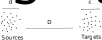
\includegraphics[width=0.5\textwidth]{introduction/degenerate_kernel.pdf}
    \caption{A set of source and target particle cluster, where the width of each cluster is significantly less than the distance separating them, $d_s, d_t \ll D$.}
    \label{fig:chpt:fmm:degenerate_kernel}
\end{figure}

Naively computed this requires $\bigO{MN}$ operations, where in general the source and target particles may correspond to the same set. The \acrshort{fmm} relies on a \textit{degenerate} approximation of the interaction kernel when subsets, or \textit{clusters}, of source and target particles are sufficiently separated as sketched in Figure \ref{fig:chpt:fmm:degenerate_kernel}. Following the discussion in \cite{kailasa2024m2ltranslationoperatorskernel} the sum (\ref{eq:chpt:fmm:laplace_potential_sum}) can be written as,

\begin{equation}
    \phi(\Xbf_i) \approx \sum_{p=1}^P \sum_{j=1}^N A_p(\Xbf_i) B_p(\Ybf_j)q(\Ybf_j), \> \> i = 1,...,M
    \label{eq:chpt:fmm:degenerate_kernel}
\end{equation}

where we call $P$ the expansion order, taken such that $P \ll N$, $P \ll M$. The functions $A_p$ and $B_p$ are defined by the approximation scheme used by a particular approach for the \acrshort{fmm}, in the original presentation the calculation,

\begin{equation}
    \hat{q}_p = \sum_{j=1}^N B_p(\Ybf_j)q(\Ybf_j)
\end{equation}

Corresponded to the coefficients of an order $P$ multipole expansion due to the source charges. Following which the potential is approximated by,

\begin{equation}
    \phi(\Xbf_i) \approx \sum_{p=1}^P A_p(\Xbf_i)\hat{q}_p, \> \> i = 1,...,M
\end{equation}

at the target particles. The approximation of the potential with this scheme can be seen to require $\bigO{P(M+N)}$ operations. The accuracy of this approximation scheme, and the error bounds provided by the \acrshort{fmm}, depends on the distance between the source and target clusters remaining large relative to their width. This condition is often referred to as an \textit{admissibility condition} in the literature. \acrshort{fmm}s therefore split the sum (\ref{eq:chpt:fmm:laplace_potential_sum}) into \textit{near} and \textit{far} components when considering arbitrary clusters of source and target particles,

\begin{equation}
    \phi(\Xbf_i) = \sum_{\Ybf_j \in \text{Near}(\Xbf_i)} K(\Xbf_i, \Ybf_j) q(\Ybf_j) +  \sum_{\Ybf_j \in \text{Far}(\Xbf_i)} K(\Xbf_i, \Ybf_j) q(\Ybf_j), \> \> i=1,..,M
    \label{eq:chpt:fmm:near_far_split}
\end{equation}

In cases where a source and target cluster can be considered \textit{admissable}, i.e. the source cluster is considered in the \textit{far field} of the target cluster such that each $\Ybf_j \in \text{Far}(\Xbf_j)$, we apply the approximation (\ref{eq:chpt:fmm:degenerate_kernel}). However, when a source and target cluster are \textit{inadmissable}, such that the source cluster is considered in the \textit{near field} of a target cluster such that each $\Ybf_j \in \text{Near}(\Xbf_j)$ we are left to evaluate the sum directly via (\ref{eq:chpt:fmm:laplace_potential_sum}).

The notion of admissability is made more concrete by reference to a data structure chosen to discretise the problem. For the \acrshort{fmm} quadtrees and octrees are commonly used in two and three dimensions respectively. These are data structures in which a $d$-dimensional bounding box is used to cover the source and target particles, and is recursively divided into $2^d$ `child' boxes. This process can be either `adaptive' or `uniform'. In the former case, the box is divided until a user defined threshold defining the maximum number of points per terminal leaf box is reached, which can lead to adjacent boxes of differing sizes and is able to closely model extreme particle distributions. In the latter case, boxes are divided such that each leaf box is of the same size, specified by a user defined parameter controlling the maximum depth of the tree.




- In order to achieve its $\bigO{N}$ complexity the \acrshort{fmm} is structured to reduce to a minimum the number of sums evaluated between inadmissable clusters.


- The full algorithm for uniform case

- sketch of complexity for full generic algorithm

- adaptive case, and why this might be useful.

- What extras does it entail. Will we consider it in this thesis?

- Define interaction lists.

- Define all operators.

- Give an algorithm sketch.

- Give complexity sketch.



\section{Computational Structure}\label{chpt:fmm:sec:computational_structure}

- The data flow is shown in Figure \ref{fig:chpt:fmm:data_flow} for all the operators for a uniform FMM in two dimensions with two levels taken in the hierarchical tree.

- In this section we map this data flow to the available parallelism on shared and distributed memory systems.

- Tree construction

    - bottom up vs top down, complexities of each approach
    - Morton vs Hilbert spatial decompositions
    - ORB as an alternative approach.
    - What are the positives and trade-offs of different spatial encodings? How much do I think it matters?
    - linked list vs linear
        - linear us, pvfmm
        - exafmm-t as an example of linked list variant.

- Interaction list access
    - Originally, based on linked lists - Anderson,
    - Move towards masking techniques, bebendorf GPU and Gumerov, as GPUs became a thing.
    - High degree of success with index pointer based techniques, us, pvfmm and exafmm.

- Runtime, Thread and Data level parallelism
    - threading model
        - tbb/rayon approach on work stealing vs openmp fork-join
    - data level
        - achieved easily if formulated with modern BLAS libraries for critical operators.

- Formulation of translation operators.
    - analytical (unrolled) formulations
        - relies on special functions, multithreading possible but manual
        - can be written as BLAS
    - algebraic
        - BLAS

Ghost data exchange of interaction lists
    - MPI
        - point to point vs collective vs neighbourhood collective
    - Runtime systems
        - BSP (ie MPI) vs task based

    - implications for caching based on granularty of tasks.

How can parallelism best be expressed?

- Unroll the FMM loop
- linearise data access for interaction lists
- ensure that as many key operations as possible can use those implementations with high flop/byte ratio and take advantage of SIMD i.e. open source FFTW/BLAS/LAPACK.

What does this mean in terms of the operators?

- Data dependency at coarsest granularty is over levels, reminiscent of V list cycle in multigrid approaches.
    - Picking this level of granularty gives the greatest flexibility to an implementer to explore options.
    - Furthermore, the P2P and recursive scheme are completely data independent and should be treated as such.

- Ensuring data locality for translations
    - i.e. it's clear that M2M and L2L can be batched over sets of siblings.
        - but can also batch over multiple sets of siblings at each level.

    - the challenge ise the M2L, where the number of accesses is as no order of magnitude larger than M2M and L2L.
    - P2P, standard techniques can be adapted due to natural parallelism over target particles. The challenge is ensuring that SIMD is used appropriately for inverse square roots, and special functions, to fully utilise cache and CPU.
    - tree and admissibility condition should be separated from the data access method
        - i.e. no matter what these are, level-wise data access is always linear over contiguous blocks.

- Parallel model that allows for tunable cache utilisation
    - this means taking advantage of 'free lunches' from open-source software for high performance, relying on BLAS/LAPACK as much as possible as well as FFT if utilised.
        - SIMD special functions, and inverse roots
    - i.e. avoid parallel models where cache coherence could be destroyed for any reason.

- Removing as much as possible into the pre-computation step.
    - i.e. separate out required data into that evaluated at runtime, and that which can be stored and cached.

- Distributed memory
    - Foundational work by Warren and Salmon.
    - naively, due to global data dependency over each level, high levels of the tree are required across the entire domain.
    - BUT the amount of data is actually extreemly small, just the multipole coefficients for long range interactions. The P2P charge data is by definition extremely local, and can be handled effectively even with point to point communication patterns which are simple.
    - modern MPI implementations can do all-reduce style operations in log(P), talk a little about this.
    - MPI 3.0 and above introduce neighbourhood communication
        - Note that, when viewed hierarchically, data exchange is local in terms of morton keys. So maps well to hierarchical neighbourhood collective communication patterns

- Software environment that allows us to mix and match all of the above, and can be a tool for both high performance simulation and algorithmic exploration.

At the end of this we have a skeleton for a high performacne FMM/hierarchical matrix

- Component diagram for high performance abstract FMM:

\begin{figure}[h]
    \includegraphics[width=\textwidth]{fmm_data_flow.png}
    \caption{Data flow for the evaluation of the potentials due to a given set of (red) source particles in the far field of a given set of (blue) target particles, in two dimensions for clarity with a uniform tree of depth two. The source particles in the near field of the target box are shown in grey.}
    \label{fig:chpt:fmm:data_flow}
\end{figure}

- Many past works have alluded to this feature of the FMM, though it is rarely expressed as such explicitly in the literature.

- Early examples include the works of Chandramowlishwaram and co-workers, who develop performance models characterising the kiFMM on various hardwares, and acknowledge the trade-off between the M2L and P2P as the key characteristic for FMM performance, and controlled by the tree depth.

- Deeper trees, synonymous with fewer particles per leaf node, and therefore smaller $U$-lists for P2P, but with more M2L.

- Shallower trees, synonymous with larger P2P and fewer M2L.

- Since then many works have focussed on expressing the data dependencies explicitly, and exposing them to special runtimes. - Proponent of task based runtime systems, as not restricted to specific algorithmic ordering of tasks removes artificial syncs, expose more native concurrency, and shorten critical path. The latter tends to restrict operations to a specific order. DAG-based dynamic runtime engines can remove artifactual synchronizations in the form of subroutine boundaries, remove artifactual orderings in the form of pre-scheduled loops, expose the native concurrency, and shorten the critical path. StarPU, Charm++ and Legion being popular runtimes.

- However as we can see there are remarkably few intra-level synchrnoisations required for the FMM, meaning that the overhead of a runtime system in comparison to ordinary multithreading based appraoches

- The principal drawback of losing this control is that though NUMA aware approaches do exist, it is significantly hardware to control data locality, which i§s critical for performance on modern architectures.

- Furthermore, most critically, the two most expensive operations of the FMM, the P2P and M2L operators, \textit{have no data dependencies} Meaning that there is amply opportunity to develop fully asynchronous implementations of these two operations, and given the optimal SIMD/SIMT structure of the P2P operation the obvious choice of operator to deploy to GPU in a heterogenous implementation.




\section{Kernel Independent Fast Multipole Methods}\label{chpt:fmm:sec:kifmm}

As mentioned the functions $A_p$ and $B_p$ in (\ref{eq:chpt:fmm:degenerate_kernel}) corresponded to explicit expansions of the Green's function in the original formulation of the FMM.

- This approach has benefits, principally it will have a very low pre-computation time for all the operators, and there have been translation operators developed for a wide range of common PDE kernels [CITE AVAILABLE KERNELS]. However, this approach also contains significant trade-offs. Very often kernel expansions rely on the evaluation of special functions for the translation operators, which can be expensive at runtime especially when large expansion orders are used.

- From a practical perspective, each kernel implementation may require kernel specific fine-tuning to achieve high performance, making a unified software framework that can tackle a range of kernels a daunting task.

- Variants of the FMM , known as `kernel Independent', take an alternative approach to explicitly constructing kernel expansions. Instead of constructing explicit expansions, they use proxies to represent the field due to the charges contained in each box, their defining feature being that they result in schemes which only rely on kernel evaluations, while remaining compatible with a wide range of elliptic PDE kernels. Notable examples include [Darve paper], [Rokhlin and Martinsson paper in 1D].

- From a software perspective, this leaves a smaller surface area of code optimisation, data organisation for the application of operators and the kernel evaluations, which together determine the performance.

- We describe in detail the approach taken in \cite{Ying:2004:JCP} as it's the method which we implement in our software.

- The principal features of this approach are its usage of equivalent charges placed on surfaces that enclose the box, and the method of fundamental solutions as its approximation scheme.

- As the scheme relies on an analysis based uniqueness argument, the kiFMM and similar schemes with some analysis used in their specification are occasionally referred to as `semi-analytical' FMMs. Though this term garners scattered use through the literature, and it is relatively common to refer to any method which does not rely on explicit analytical expansions of the interaction kernel as an `algebraic' method.

- Review all translation operators

- How is pinv constructed? What limits the accuracy of these factors in the original kiFMM, how was this rectified by kiFMM (pvFMM)

- Comment on storage requirements for Laplace and Helmholtz kernels in 3D.

- Comment on what can be precomputed and cached.

- Comment on specification of the operators as matrix-vector operations.

- Brief comment on M2L acceleration of the original spec of this method, ie. why was SVD based compression and BLAS abandoned and FFT favoured?

- Expected convergence behaviour, are the multipoles also exponentially converging with expansion order?

One of the big advantages of using outer and inner sphere approximations is the simplicity of the process of combining them. This is in contrast to the complicated formulas that must be used if the approximations are based on spherical harmonics.


\section{Oscillatory Fast Multipole Methods}\label{chpt:fmm:sec:oscillatory}

The crucial feature of the Laplace kernel (\ref{eq:chpt:introduction:laplace_kernel}) is the fact that far-field interactions (\ref{eq:chpt:fmm:near_far_split}) can be considered `low rank', and therefore amenable to compression. Importantly for (\ref{eq:chpt:introduction:laplace_kernel}) the rank of a given interaction between two boxes is scale invariant, and only depends on their relative positions.

However, for problems described by the Helmholtz kernel,

\begin{equation}
    K(\mathbf{x-y}) = \begin{cases}
        \frac{i}{4} H_0^{(1)}(k |\mathbf{x-y}|)  \text{, $d$ = 2}\\
         \frac{e^{ik |\mathbf{x-y}|}}{4\pi |\mathbf{x-y}|}  \text{, $d$ = 3}
    \end{cases}
    \label{eq:chpt:fmm:helmholtz_kernel}
\end{equation}

where $d$ is the spatial dimension, $\Xbf, \Ybf \in \Rd$, $k$ is the wavenumber, $H_0^{(1)}$ is the Hankel function of the first kind of order 0. The rank of interactions is no longer scale invariant, and indeed grows with box size. To see why this may be, consider the case for $d=3$. From theorem 2.11 in \cite{colton1998inverse}, we can express the Helmholtz kernel as a separable series,

\begin{equation}
    \frac{e^{ik|\Xbf - \Ybf|}}{4\pi |\Xbf - \Ybf|} = ik \sum_{p=0}^\infty \sum_{-p}^p h_p^{(1)}(k|\Xbf|) Y_p^m(\frac{\Xbf}{|\Xbf|})j_p(k|\Ybf|) \overline{Y_p^m(\frac{\Ybf}{|\Ybf|})}
\end{equation}

Where $k$ is the wavenumber, $Y_p^m$, for $m=-n,...,p$ $p=0,1,...$ are set of orthonormal spherical harmonics, and $|\Xbf| > |\Ybf|$, $j_p$ is the spherical Bessel function of order $p$ and $h_p^{(1)}$ is the spherical Hankel function of the first kind of order $p$.

In which case, an expression of the form (\ref{eq:chpt:fmm:degenerate_kernel}) for the Helmholtz potential evaluated at a set of $M$ target particles due to a set of $N$ source particles

\begin{equation}
    \phi(\Xbf_i) \approx \sum_{p=1}^P \sum_{m=-p}^p \sum_{j=1}^N A_p(x_i) B_p(y_j) q(y_j), i=1,...,M
\end{equation}

where we've truncated the expansion to $P$ terms, known as the expansion order, and $A$ and $B$ are functions of the target and source particle positions only, respectively. We see that in this case for increasing expansion order, the number of terms in the sum grows quadratically. Though a demonstration is out of scope for this thesis, we mention that the number of terms $P$ required to observe convergence in the above sum is proportional to $kD$

\begin{equation}
    P \approx kD
    \label{eq:chpt:fmm:p_kd}
\end{equation}

Some work for schemes that rely on the \acrshort{mfs} is presented in \cite{barnett2008stability}. Therefore, in the \acrshort{fmm} for oscillatory problems interactions between boxes can be seen to have ranks growing quadratically, proportionally to $(kD)^2$, for increasing box size in 3D.

For schemes based on \acrshort{mfs} as the \acrshort{kifmm} used in our software, the quadratic relationship between rank growth and box size is observed by noting that the condition for convergence (\ref{eq:chpt:fmm:p_kd}) corresponds to a fixed number of points per square wavelength (in 3D), therefore the rank, which is proportional to the number of points used to discretise the equivalent surfaces, can be seen to grow quadratically with increasing box size.

Previous approaches to handle this for analytical \acrshortpl{fmm} can be technically complex

However, there has been some significant results in developing `kernel independent' approaches for oscillatory problems. The resulting schemes closely mirror the \acrshort{kifmm}




% In order to handle this, past implementations rely on so called `diagonal forms' of the translation apparatus when the \acrshort{fmm} can be considered to be in its high frequency regime.

% The implementation of these schemes is complex, and few optimised softwares exist in the open source. Indeed, kernel independent variants have also been developed. These rely on the so called `directional low rank' property of the Helmholtz kernel.

% ... basic scheme of directional low-rank

% The basic scheme is extremely similar to the kernel independent \acrshort{fmm}, save for the additional loop over cone directions.

% However, there is no actively maintained open-source software available.

% Considering this, we consider to what extent the machinery of the \acrshort{kifmm} can be re-used for moderate frequency problems. How high can wavenumber be increased, before the lack of linear scaling leads to poor overall runtimes? We are able to test this as in our implementation we are able to tune expansion order by level.

% However, if one can increase $P$ with decreasing tree level, for trees of moderate depth and moderate wavenumbers $k$, as long as the \acrshort{p2p} and \acrshort{m2l} implementations are optimal, we demonstrate that it is possible to achieve high practical performance with the relatively simple machinery of the \acrshort{kifmm}.




\section{Distributed Memory Fast Multipole Methods}\label{chpt:fmm:sec:distributed}

Supercomputers are usually defined as massively parallel machines characterised by hundreds to thousands of individual nodes comprising of individual hardware pieces which communicate via a network. In this context memory movements, now between compute nodes, are of even greater practical relevance

- Network topologies, NVLink and other RDMA technologies that are emerging.
- Rate of improvement in bandwidth/latency on network vs DRAM.

Minimising communication is crucial
- Ibeid communication costs, and how these can be simplified.


- How are FMMs distributed for distributed memory?

- Focus is on the maximal reduction in communication.

- what communication can and cannot be avoided?

- How the local/global split in terms of tree gives rise to optimal communication scheme.

- What simplifying assumptions can we take for most pre-exascale systems?

- Avoid sorting of Morton keys/point data, the local/global split gives us a way to statically partition tree across available resources - simplifying assumption if work with ncpu = pow(8).
- Not restricted to this, but makes threading simpler for local FMMs.

- Optimal implementation of MPI primitives for common data sizes.

- What will probably not work approaching exascale?
- the gather operation over all processes required for multiple steps of this algorithm - ghost exchange, multipoles at local root on nominated processor. How can these problems be addressed? Do they even matter for the problem sizes we're concerned with?

- Bandwidth and latency complexity estimates for communication approaches
- Bandwidth
    - total data transfer, transfer per process, scaling with PARFOR
- latency
    - Number of communication steps,
    - scaling with P



\section{Algorithm Zoo}\label{chpt:fmm:sec:algorithm_zoo}

Having described the key intuition behind the \acrshort{fmm} for oscillatory and non-oscillatory kernels, as well as our variant of interest the \acrshort{kifmm} of Ying and co-workers. We use this section to describe a few of the vast numbers of variant approaches to compute the \acrshort{fmm}, and unify the literature on \acrshort{fmm} with that of the closely related \textit{hierarchical matrices}, or $\H$ matrices for short.

The \acrshort{fmm} and related methods principally vary with respect to their admissability criterion, method of field approximation, and underlying hierarchical data structure used.

Often \acrshortpl{fmm} and related methods are grouped roughly into three categories

\textbf{Analytic}, where kernel dependent expansions are used to approximate the fields. Original method, extended since then to a range of PDE kernels, including oscillatory problems described by time harmonic maxwell and helmholtz equations. For example originally, a multipole expansion was used. In 2D these take the form of simple coefficients, in 3D for Laplace already have to deal with spherical harmonic basis.

\textbf{Semi-Analytic}, examples include the kiFMM and the bbFMM, here only kernel evaluations are used however analytical properties are required in the construction of the fictitious surfaces on which the methods rely. examples include the kiFMM of \cite{Ying:2004:JCP} and also the black box FMM \cite{fong2009black}.

\textbf{Algebraic}, purely rely on kernel evaluation, Martinsson and Rokhlin 2011 \cite{martinsson2007accelerated}

- Analytical FMMs
- different expansion representations, and their impact on complexity, table from yokota paper,
- comment on complexity vs real implementation (special functions computation, for some kernels there are simplifying approaches e.g. Gumerov real Laplace expansions)

- Comment on lack of unified comparison in the literature

The line between `algebraic' and `semi-analytic' is fuzzy in practice, as the nature of the computations have an extremely close correspondence, and in the example of the kiFMM of \cite{Ying:2004:JCP} equivalent up to a choice of discretisation to the purely `algebraic' $\Htwo$ matrix scheme.

When it comes to practical performance there is a gap in the literature in terms of a direct comparison between these rough approaches. Many of them achieve optimal asymptotic complexities, however practical performance depends principally on components that appear as constants in complexity estimates - related to memory accesses, and optimal vectorisation and parallelisation where possible.

Indeed, the \acrshort{fmm} can be seen to be a special case of the more general hierarchical matrices, or $\H$ matrices for short.

- Generally considered that low-order analytical and high-order algebraic approaches, for performance however this is not actually known.

- analytical requires evaluation of special functions, what does this look like on modern architectures? Surely this is not a preferred operation, and will not be going in to the future.

Common $\H$ matrix formats are summarised in table [Ambikasaran table], indeed we see that the FMM is actually of class $\Htwo$. Though often written about in different contexts, and by different geographically disparate communities, algebraic variants of the the \acrshort{fmm} can be seen to be equivalent to methods for $\Htwo$ matrices, the principal difference being that algebraic \glspl{fmm} are commonly defined using quad/octrees whereas $\Htwo$ matrices rely on the more generic `cluster tree' approach that works directly with matrix entries.

- How are analytical expansions defined, 2D Laplace example, note and references on 3D laplace example.
    - private note on how these derivations are found.

- Note on admissibility, how it defines a broad class of FMM matrices, table of related matrix types with different rank structure and admissability criterion

- HSS, HBS, $\H$, $\Htwo$ exactly where does the FMM fit in.

- What is the expected complexity of matrix vector product, how do they differ (nested vs non-nested bases).

- How are off diagonals approximated? Linear algebra. e.g. SVD/ACA/CUR decompositions vs analytical expansions.

- Relative costs of computing these, precomputation is expensive in general compared to FMM which uses analytical expansions and minimal precomputation costs.

- Alternative to geometry captured by oct/quadtree. ORB could also be used for the FMM.

- But rely on cluster tree and cluster block trees over the matrix indices.

This is achieved with a hierarchical discretisation of the problem domain, often a \textit{quadtree} in two dimensions and correspondingly an \textit{octree} in three dimensions.

- trees define admissability from geometry for FMM, note on alternative approaches such as ORB.

- can control interaction list in different ways by using control parameter in ORB.

- Control of the interaction list is an optimisation used in stencil based approaches, more recent efforts like the Yesypenko paper, older approaches like Gumerov and the 8,4,2 method mentioned in the Yokota summary paper.

- These data structures are generated by creating a bounding box that covers the source and target particles, which without loss of generality may correspond to the same set. This box is then recursively sub-divided into \textit{child boxes} of equal size.

- There is relatively little work directly contrasting the relative merits of different approaches for constructing \acrshortpl{fmm}. Yokota et. al \cite{yokota2015fast} provide some analysis, attempting to bound the vast literature on \acrshort{fmm} and related methods, however stop short of rigorous benchmarks. Indeed, direct software benchmarks between different groups and approaches can be flawed for numerous reasons, principally whether or not a given implementation was optimised for optimal hardware use or simply for demonstrative purposes. Furthermore, Yokota et. al only compare their analytical implementation of the \acrshort{fmm} for Laplace kernels in 3D with an implementation for HSS matrices, which though of the same asymptotic complexity, have completely different scaling properties in 3D.

- A general rule of thumb has so far been that algebraic methods perform better at high order, meanwhile analytical methods are more suitable for low order. It's understandable to see where this point of view comes from. The translation operators for analytical \acrshortpl{fmm} take the form of very short sums, potentially involving special functions. The practical evaluation of which though highly optimised, are inherently expensive in terms of \acrshortpl{flop} for high order evaluations. On the other hand, kernel independent approaches rely only on the evaluation of matrix blocks that are constructed via kernel evaluation, and therefore are easy to express as \acrshort{blas} operations.

- As a point of direct comparison, we present the scaling on a single node of computing the Laplace problem in 3D on a range of modern softwares. We compute the problem on the surface of a sphere, taking increasingly fine discretisations of its surface, a sphere is chosen as a range of modern \acrshort{fmm} and $\Htwo$ matrix software is optimised for \acrfull{bem} applications

Alternative $N$-body approaches, there has been limited work except a landmark study \cite{gholami2016fft}, again the asmpyotic costs of these competing approaches is important

- Asymptotic costs of competing approaches include $\bigO{N \log{N}}$ for the \acrshort{fft} and $\bigO{N}$ for multigrid

- The FFT has been shown to have $\bigO{P^{1/d}}$ communication complexity, with $\bigO(\log{P})$ for multigrid. Recently the \acrshort{fmm} has also been shown to have $\bigO{\log{P}}$ communication complexity, and therefore the trade-offs between different approaches are significantly harder to contrast.

- FFT is generally preferred for problems with uniform resolution, multiscale features are somewhat better handled by the FMM and multigrid in theory. However, interpolation of non-uniform features can be handled efficiently with effective \acrshort{simd} and caching optimisations.

- But the most important costs are related to data handling, and unique again to a specific implementation.

\begin{table}[ht]
    \centering
    \caption{Comparison of Expansion Types, adapted from \cite{Yokota2013} and expanded with more recent variants and estimates.}
    \begin{tabular}{lcc} % lcc means left-align the first column, center-align the other two
    \toprule
    \textbf{Approximation Scheme (+ M2L Scheme)} & \textbf{Storage} & \textbf{Naive Arithmetic} \\
    \midrule
    Cartesian Taylor & $\bigO{P^3}$ & $\bigO{P^6}$ \\
    Cartesian Chebyshev (+ Direct Compression) & $\bigO{P^3}$ & $\bigO{P^6}$ \\
    Spherical Harmonics & $\bigO{P^2}$ & $\bigO{P^4}$ \\
    Spherical Harmonics (+ `point and shoot') & $\bigO{P^2}$ & $\bigO{P^3}$ \\
    Spherical Harmonics (+ FFT) & $\bigO{P^2}$ & $\bigO{P^2 \log{P}}$ \\
    Planewave & $\bigO{P^2}$ & $\bigO{P^3}$ \\
    Equivalent Charges & $\bigO{P^2}$ & $\bigO{P^4}$ \\
    Equivalent Charges (+ FFT) & $\bigO{P^3}$ & $\bigO{P^3 \log{P}}$ \\
    Equivalent Charges (+ Direct Compression) & $\bigO{P^2}$ & $\bigO{k^2 \cdot P^2}$ \\
    \bottomrule
\end{tabular}
\end{table}





\section{Available Software}\label{chpt:fmm:sec:software}

Despite the intensity of developments over the last decade, the software landscape is fragmented for \acrshortpl{fmm} and related methods.

- What software exists, and which approaches do they use?

The lack of re-usable subcomponents slows down algorithmic innovation. For example, there are numerous implementations of \acrshort{simd} vectorised Green's functions, community software building has been poor.

We show the performance of some of the main implementations below for Laplace and Helmholtz.

Additionally, implementations are designed to demonstrate the performance of specific approaches and algorithms. It is exceptionally hard to swap algorithmic approaches, hardware and software backends. For example ExaFMM-T / ExaFMM are re-implementations of the entire FMM algorithm, where much of the underlying machinery for algorithm deployment is identical - it's just the metadata required for the operators and the approximation scheme which is different. Yet these are both long, overlapping, and complex libraries.

- No software aims to make any guarantee about performance, but neither do they expose subcomponents to users. At least one fo these should be done so that community efforts can begin in earnest, and software lives beyond a PhD research project.

To the best of our knowledge, no other open-source FMM software have the ability to vary expansion order by level.




    \chapter{Comparing Field Translation Approaches for Kernel Independent Fast Multipole Method}\label{chpt:field_translation}
\thispagestyle{chaptertitle} % Force the fancy style on this page


\begin{center}
    \textit{The content in this chapter is adapted from the material first presented in \cite{kailasa2024m2ltranslationoperatorskernel} }
\end{center}

- Review of approaches, success and failures, and what works in the context of modern software and hardware systems.

- What are important trends, and what have we actually done.

    \chapter{Modern Programming Environments for Science}\label{chpt:programming_for_science}
\thispagestyle{chaptertitle} % Force the fancy style on this page

% \section{Developing Scientific Software}\label{chpt:1:sec:0}

Scientific software development presents a unique set of challenges. Although development teams are frequently small, they are tasked with producing highly optimised code that must be deployed across a myriad of hardware and software platforms. Moreover, there is a pressing need for comprehensive documentation and rigorous testing to ensure reproducibility. Given that many of these softwares arise within doctoral programs or other short-term projects, there is a tendency to tailor software development to showcase a specific project's objectives. Whether that be to demonstrate a convergence result of a specific methodological improvement, or offer a new benchmark implementation of an algorithm. Consequently, once the principal results are achieved these software projects often become orphaned, lack compatibility with a range of development platforms, or aren't adaptable to related challenges and subsequent research by other teams.

A recent survey of 5000 software tools published in computational science papers featured in ACM publications found that repositories for computational science papers had a median active development span of a mere 15 days. Alarmingly, one third of these repositories had a life cycle of less than one day \cite{hasselbring2020open}. Implying that upon the publication of the affiliated paper, software typically gets abandoned or, at best, receives private maintenance. This trend underscores the challenge of dedicating sustained resources in an academic setting to software upkeep, even when such maintenance is vital for reproducibility. It may also hint at a deficiency in professional software engineering expertise among computational researchers whose principal expertise lies elsewhere.

Therefore, confronting the challenge of developing maintainable research software relies on the choice of programming environment. Developers need to have a frictionless system for testing, documenting, using existing open-source solutions and building extensions to their code. Software design has to be general enough to extend to new algorithmic developments, but also malleable enough for external developers and users to adapt software to new usecases as well as their own needs. Building software for diverse software environments and target architectures should also be painless as possible to encourage large-scale adoption. Additionally, domain scientists who are typically not experienced in low-level software development require interfaces to familiar high level languages, which must be easy to maintain for core-developers.

In the early stages of this research project we experimented with Python, a high-level interpreted language, that has become a de-facto standard in data-science and numerical computing for a wide variety of domain scientists. Recent years have seen the development of tools that allow for the compilation of fast machine-code from Python, allowing for multi-threading, and the targeting of both CPU and GPU architectures \cite{lam2015numba}. This approach takes advantage of the LLVM compiler infrastructure for generating fast machine code from Python via the Numba library, and is similar to other approaches to creating fast compiled code from high-level languages such as Julia \cite{bezanson2017julia}. We built a prototypical single-node multithreaded implementation of a fast algorithm, the fast multipole method (FMM), in Python to test the efficacy of this approach. However, we found that for complex algorithms writing performant Numba code can be challenging, especially when performance relies on low-level management of memory \cite{kailasa2022pyexafmm}. We summarise this experience in section \ref{chpt:1:sec:1}. We identified Rust, a modern low-level compiled language, as a promising programming environment for our software. Rust has a number of excellent features for scientific software development, most notably the introduction of a `borrow checker', that enforces the validity of memory references at compile time preventing the existence of data races in compiled Rust code, as well as its runtime `Cargo', which offers a centralised system for dependency management, compilation, documentation and testing of Rust code. We summarise Rust's benefits, as well as notable constraints, in section \ref{chpt:1:sec:2}. We conclude this chapter by noting that language and compiler development for scientific computing is an active area of research, in section \ref{chpt:1:sec:3} we contrast Rust with emerging programming environments for scientific software.
% - Summary of the algorithm's logic - and the low rank assumption behind its power. 

- Overview of the choices that can be made: translations, expansions, etc.

~ 2 pages
% \section{Introducing Rust for Scientific Software}\label{chpt:1:sec:2}


% \section{Emerging Developments}\label{chpt:1:sec:3}

Despite the above criticisms, high-level languages as tools for high-performance scientific computing remain an intense area of research and development. `Mojo' is a new programming language, along with a compiler. It's built as a superset of Python, specifically with the two-language problem in mind. Additionally, it attempts to address the `three language problem', whereby languages also target exotic hardware such as GPUs and TPUs \cite{Lattner2023Mojo}.
    
This is achieved by building on the MLIR compiler infrastructure. MLIR can be thought of as a generalisation of LLVM, catering to CPUs, GPUs, and novel ASICs for AI. The team chose to develop around Python to leverage its extensive existing user base in computational and data sciences.

Currently, Mojo remains a closed-source language and is actively being developed by its parent company, Modular. Thus, even though it appears promising, it's not yet in a state suitable for experimentation. Nevertheless, Mojo showcases the potential of a future programming environment that might definitively `solve' the problems developers face when selecting a programming environment for academic software.

    \chapter{Designing Software for The Fast Multipole Method}\label{chpt:designing_software_for_fmm}
\thispagestyle{chaptertitle} % Force the fancy style on this page

\section{Fast Multipole Methods}

\section{Kernel Independent Fast Multipole Method}

\section{Computational Issues}

Bottlenecks in shared and distributed memory

Tree Construction

M2L kernels

P2P kernels (cite out work)


\section{Software Issues}

JOSS paper

Data oriented design for kiFMM-RS

Traits for flexibility

Code generation for multiple targets

Flexible backends

\section{Performance Model}



\section{Distributed FMM}

\section{Helmholtz FMM}


% \section{The Fast Multipole Method}


% \section{Algebraic FMM Variants}\label{chpt:2:sec:1}

In its original analytical form the applicability of the FMM is limited by the requirement for an explicit multipole and local expansions, as well as a restriction to matrix vector products. Subsequent decades saw the development of `algebraic' analogues to the original algorithm. These methods are similarly based on a hierarchical partitioning, whether that be of the point data using a recursive tree as with the original FMM \cite{Ying:2004:JCP,fong2009black}, or by operating on the matrix implied by the FMM's algorithmic structure directly \cite{hackbusch1999sparse,borm2003introduction,chandrasekaran2007fast}. The latter methods are collectively known as $\mathcal{H}$-matrix methods. Representing the FMM operation in this way has allowed extension of the FMM to other matrix computations, such as matrix-matrix products, as well as approximations of its inverse \cite{ambikasaran2014inverse}. Notably, many of these methods don't necessarily rely on explicit multipole/local expansions for approximating fields as in the original FMM in the previous section. Examples such as the `kernel independent FMM' (kiFMM) of Ying and co-authors instead relies on the method of fundamental solutions to approximate the fields and requires only evaluating kernel values, and is applicable to a wide range of kernels from second-order linear non-oscillatory elliptic PDEs with constant coefficients such as the Laplace equation. This approach relies on some analytic considerations, however methods also exist which are interpolatory - such as the `black box FMM' (bbFMM) of Fong and Darve \cite{fong2009black}, which similarly only relies on kernel evaluations and a Chebyshev scheme to approximate fields.

In our software we choose to implement the kiFMM of Ying and coauthors, which we explain in detail below adapting the discussion from Section 3 of \cite{Ying:2004:JCP}. This method shares advantages with other algebraic FMM methods, of generality to a large class of problems, as well as opportunities to optimise computer implementations we explore in Section \ref{chpt:2:sec:1}. This approach relies on a spatial discretisation of the problem domain via an quad/octree as in the original FMM, as well as the method of fundamental solutions (MFS) for approximating the fields from point charges/masses. This method has been demonstrated to scale well on shared \cite{wang2021exafmm} as well as distributed memory \cite{malhotra2015pvfmm} systems, achieve similar accuracy to the analytical variant, with relatively low pre-computation required. The underlying data structure of the quad/octree has been a significant area of research and development, with established high-performance methods for their construction in shared/distributed memory environments \cite{sundar2008bottom,sundar2013hyksort,BursteddeWilcoxGhattas11}.

Consider the kernels for second-order constant coefficient non-oscillatory PDEs, such as that of the Laplace equation in (\ref{eq:chpt:2:sec:0:laplace_kernel}). Such kernels satisfy the underlying PDE everywhere except the singularity location, and are smooth away from this singularity. These problems admit a unique solution for interior/exterior Dirichlet boundary value problems (see Appendix \ref{app:laplace_bvp} for a demonstration of this for the Laplace equation). The authors of \cite{Ying:2004:JCP} rely on the smoothness and uniqueness of the Dirichlet boundary value problems as basic properties to develop their FMM formulation. The problem setting as before is the calculation of (\ref{eq:chpt:2:sec:0:fmm_problem}) for the Laplace kernel, for a set of $N$ point sources $y_i$, $i = 1...N$, which we will associated with $N$ source densities $q_i$, an target locations $y_j$, $j=1...M$. As before, the source and target locations may coincide. We use an index set $I^B_s$ and $I^B_t$ to identify the sources and targets we are considering in a particular interaction. We assume that our problem is in $\mathbb{R}^3$, however the exposition is essentially the same as in $\mathbb{R}^2$.

Assuming that we have constructed our hierarchical tree partitioning, which may be adaptive, the first step is to approximate the fields due to particles contained in each leaf box. We specify more concretely that for a given box, $B$, its `near field range', $\mathcal{N}^B$, is the set of 27 boxes at the same level of a tree which are adjacent to it, i.e. they share a corner, face or edge as well as $B$ itself. Its `far field range', $\mathcal{F}^B$, is simply the boxes which are the complement of this.

We approximate the potential in $\mathcal{F}^B$ from the source densities $\{ q_i : i \in B \}$ in $B$ using the potential from an \textit{equivalent density distribution}, $q^{B, u}$, supported at prescribed locations $y^{B, u}$ (see the left box in Figure \ref{fig:chpt:2:sec:1:multipole_local}). Where $q^{B, u}$ is called the \textit{upward equivalent density} and $y^{B, u}$ is called the \textit{upward equivalent surface}. This amounts to representing the potential with a `single layer' potential \cite{Kress2014},

\begin{flalign}\label{eq:chpt:2:sec:1:single_layer_potential}
    \phi(x) &:= \int_{y \in y^{B, u}} q^{B, u}(y)K(x, y) ds(y), \> \> x \in \mathbb{R}^3 \setminus y^{B, u}
\end{flalign}

To guarantee the smoothness of the potential produced by $q^{B, u}$ in the far-field, its support $y^{B,u}$ must not overlap with $\mathcal{F}^B$ due to the singularities in this integral from the kernel function when evaluated on the equivalent surface. Secondly, we note that the equivalent surface must enclose $B$ from the definition of the single layer potential \cite{Kress2014}. We see that the equivalent surface must be placed in between the box and the boundary of $\mathcal{F}^B$.

The potential induced by our equivalent densities and upward equivalent surface satisfies the Laplace equation. Therefore, due to the uniqueness of the exterior Dirichlet boundary value problem for this kernel (as well of kernels of a similar type), we reason that the potential calculated using (\ref{eq:chpt:2:sec:0:fmm_problem}) directly from the source particles must be equivalent to that calculated using (\ref{eq:chpt:2:sec:1:single_layer_potential}) in $\mathcal{F}^B$, or anywhere between $y^{B, u}$ and $\mathcal{F}^B$. Thus we place an intermediate surface called the \textit{upward check surface} between $\mathcal{F}^B$ and $y^{B, u}$, denoting it with $x^{B, u}$. The potential computed at this surface is called the \textit{upward check potential}, which we denote by $\phi^{B, u}$.

We write this as,

\begin{flalign}\label{eq:chpt:2:sec:1:multipole_appx}
    \int_{y^{B, u}} K(x, y) q^{B, u} dy = \sum_{i \in I^B_s} K(x, y_i)q_i = \phi^{B, u}\> \>, \text{for any } x \in x^{B, u}
\end{flalign}

Solving for the equivalent densities is an equivalent method of approximating the far-field potential induced by the points in $B$. We identify this with a \textit{multipole expansion}. Now considering source densities which are not contained in a box $B$ (see right box of Figure \ref{fig:chpt:2:sec:1:multipole_local}) but in its $\mathcal{F}^B$, we can construct an equivalence for local expansions using a similar approach. To ensure the existence of the \textit{downward equivalent densities} $q^{B, d}$, the \textit{downward equivalent surface}, $y^{B, d}$, must be located between $B$ and $\mathcal{F}^B$ and the potentials generated by the source points are matched to those generated by the equivalent points on a \textit{downward check surface}, $x^{B, d}$ that encloses the box and is itself enclosed by $y^{B, d}$ in order to calculate a \textit{downward check potential} $\phi^{B, d}$.

\begin{flalign}\label{eq:chpt:2:sec:1:local_appx}
    \int_{y^{B, d}} K(x, y) q^{B, d} dy = \sum_{i \in I^{\mathcal{F}^B}_s} K(x, y_i)q_i = \phi^{B, d} \> \> \text{for any } x \in x^{B, d}
\end{flalign}

In $\mathbb{R}^3$ the authors chose to represent the equivalent and check surfaces as cubes, with the equivalent/check points arranged regularly over the surfaces. We choose the same as it leads to implementation benefits when designing the field translation operators (see Section \ref{chpt:1:sec:2} for how we take advantage of this).

\begin{figure}
    \centering
    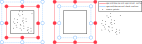
\includegraphics[width=\textwidth]{ch_2/p2m.pdf}
    \caption{ We illustrate the equivalent/check surfaces and associated boxes in $\mathbb{R}^3$, where we show a corresponding cross section. In the first figure, we illustrate the situation in the `P2M' operation, where we are trying to construct an approximation to the potential generated by points in a box by matching it to that generated by a set of equivalent density points placed on a fictitious surface enclosing it. In the second figure we illustrate the `P2L' operation, where we are now trying to construct an approximation to the  potential generated by points in a box's far-field within the box.}
    \label{fig:chpt:2:sec:1:multipole_local}
\end{figure}

Equations (\ref{eq:chpt:2:sec:1:multipole_appx}) and (\ref{eq:chpt:2:sec:1:local_appx}) are examples of \textit{Fredholm integral equations of the first kind}, the inversion of which is ill-posed. To solve these equations, we must first discretise, for which we made use of the \textit{Method of Fundamental Solutions} (MFS), a technique whereby the potential is approximated by a linear combination of kernel function evaluations at a set of discrete points with associated densities,

\begin{flalign}\label{eq:chpt:2:sec:1:mfs}
    \phi(x) \approx \phi^N(x) = \sum_{y_i \in y^{B, u}} K(x, y_i) q_i
\end{flalign}

Where $N$ denotes the number of equivalent points of density are placed on the equivalent surface. To see how this approximates the single-layer operator we used above to calculate the potential we simply replace the continuous density functions in (\ref{eq:chpt:2:sec:1:single_layer_potential}) with $\sum_{j=1}^N q_i \delta(y-y_j)$, recovering (\ref{eq:chpt:2:sec:1:mfs}). Writing (\ref{eq:chpt:2:sec:1:multipole_appx}) or (\ref{eq:chpt:2:sec:1:local_appx}) in matrix form reflecting the discretisation via MFS,

\begin{flalign}
    K q = \phi
\end{flalign}

We can solve the problem with Tikhonov regularisation,

\begin{flalign}
    q = (\alpha I + K^* K)^{-1}K^*\phi
\end{flalign}

which converts it into a \textit{Fredholm integral equation of the second kind} which are well-posed. The regularisation parameter $\alpha$ is found empirically. Computing (\ref{eq:chpt:2:sec:1:multipole_appx}) is equivalent to the $T^{P2M}$ operator described in the previous section for the analytical FMM, (\ref{eq:chpt:2:sec:1:local_appx}) is equivalent to an $T^{P2L}$ operator which was not explicitly described. As before, these operators take a set of charges, and create expansions that allow us to evaluate their potential in the far-field, however the method of creating the expansions is clearly significantly different. The most notable change being that our above formulation \textit{does not require explicit analytical expansions of the kernel function}, only making use of kernel evaluations.

To complete the kiFMM we need analogues to the field translation operators, $T^{M2L}$, $T^{M2M}$, $T^{L2L}$. We illustrate the required surfaces for each of these operators in Figure \ref{fig:chpt:2:sec:1:translations}. For $T^{M2M}$ we must translate the upward equivalent density of $A$ to the centre of its parent box $B$, solving the following equation for $q^{B, u}$,

\begin{flalign}
    \label{eq:chpt:2:sec:1:m2m}
    \int_{y^{B, u}} K(x, y)\phi^{B, u}(y)dy = \int_{y^{A, u}}K(x, y)\phi^{A, u}(y) dy, \> \> \text{for all } x \in x^{B, u}
\end{flalign}

As before, $y^{A, u}$ must enclose the child box $A$. During the downward pass, we must evaluate the downward equivalent density, corresponding to a local expansion, from the multipole expansions of non-adjacent boxes in $B$'s parent neighbour's children. We similarly write down for $T^{M2L}$,

\begin{flalign}
    \label{eq:chpt:2:sec:1:m2l}
    \int_{y^{B, d}} K(x, y)\phi^{B, d}(y)dy = \int_{y^{A, u}}K(x, y)\phi^{A, u}(y) dy, \> \> \text{for all } x \in x^{B, d}
\end{flalign}

Finally, the local expansions of each box $B$ must be translated to the centre of each of its children $A$,

\begin{flalign}
    \label{eq:chpt:2:sec:1:l2l}
    \int_{y^{B, d}} K(x, y)\phi^{B, d}(y)dy = \int_{y^{A, d}}K(x, y)\phi^{A, d}(y) dy, \> \> \text{for all } x \in x^{B, d}
\end{flalign}

For each of these translation operators we use the discretisation based on MFS discussed above, and solve using Tikhonov regularisation. For the  $T^{L2P}$, $P2P$ and $T^{M2P}$ operators we simply use direct kernel evaluations at the target points with respect to the equivalent densities represented by the multipole or local expansion coefficients or the true densities at the source points.

\begin{figure}
    \centering
    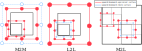
\includegraphics[width=\textwidth]{ch_2/translations.pdf}
    \caption{ As in Figure \ref{fig:chpt:2:sec:1:multipole_local}, we illustrate the translations as cross sections of the surfaces, which are cubes in $\mathbb{R}^3$.}
    \label{fig:chpt:2:sec:1:translations}
\end{figure}


% - Summarise pyexafmm paper, and what it hoped to discover - Can we use JIT compilers to build cse applications? Answer, probably not.

- Give an overview of the constraints on program design.

- Conclude with idea that an alternative is necessary, but going back to C++ isn't the right option.

- List what we ideally want from a language for scientific computing. Speed is one thing, but we also want maintainability, easy testing, building on different environments, Python...


% \section{Building for Re-Use in Fast Algorithm Software}\label{chpt:2:sec:3}

High performance software for the core data structure of quad/octrees is essential to all fast algorithms. Indeed, these hierarchical discretisations are found across scientific computing applications [REFERENCES FOR APPLICATIONS OF TREES]. Similarly, methods for sparsifying the $T^{M2L}$ operator, whether that be via an SVD or FFT, can also be re-used in the implementation of fast direct solvers, or alternative algebraic FMMs such as the bbFMM of Fong and Darve \cite{fong2009black}. The same is true of software for evaluating kernel functions in $P2P$ operator. We identify the decoupling of these separate components to be rare in other softwares for fast algorithms \cite{malhotra2015pvfmm,wang2021exafmm,h2lib2016github}, which are often presented as a monolith to users, making it difficult for developers to extend or adapt this software to their use-case.

Our software is designed to be de-coupled as independent sub-components. We achieve this using Cargo, which allows the development of `workspaces'. This is a modern language feature, without a direct parallel provided in competitors such as Fortran or C/C++. With workspaces, all sub-packages (known as `crates' in Rust) share a common build directory - speeding up build compile times, and ensuring that dependencies are uniformly versioned across all crates, specified by a root level TOML dependency file. Indeed, crates within a workspace can be specified to be binaries, libraries, or both, allowing for sub-components to easily be deployed independently or used as a dependency by a downstream developer.

- Explain in detail how traits work to specify shared behaviour in comparison to oop

- what are the trad-offs with traits (orphan rule)
- what are the benefits (implement for non-local types)
    - e.g. developers can change our kernel/translation implementations
    - implement open/close principle - composition
    - diamond problem, e.g. multiple inheritors which implement a base class, is not a thing.
    - all the polymorphism is compile time (runtime via trait objects?)
        - I don't think this is a big criticism really, relatively similar.
    - FMM/Fast algorithms naturally fall into sub-components
        - e.g. trees, translation operators, share large parts of algorithm structure.
        - packaging data with behaviour as with oop is difficult, as data structures are often very different.
            - much easier to implement a trait over a type, vs creating a completely new class for each type
                - clearer to glue together using trait contracts.



- How the design of, say translation operators, is relatively generic and plug and play.
- same for P2P, via traits as well, can plug in a GPU implementation say.


    \chapter{Numerical Experiments}\label{chpt:experiments}
\thispagestyle{chaptertitle} % Force the fancy style on this page


\section{Laplace}\label{experiments:sec:laplace}
\subsection{Single Node}\label{chpt:experiments:sec:laplace:sub:single_node}

\subsection{Multi Node}\label{chpt:experiments:sec:laplace:sub:multi_node}

- Weak scaling, communication vs computation time breakdown.

- Load balance discussion, does it matter for the distributions tested?

- Discussion on impacts of bandwidth and latency, and potential for async.

- Trade-off sort methods.


\section{Helmholtz}\label{chpt:experiments:sec:helmholtz}

\subsection{Single Node}\label{chpt:experiments:sec:helmholtz:sub:single_node}

Simple benchmark for low $k$

\subsection{How High Can $k$ Go?}\label{chpt:experiments:sec:helmholtz:sub:high_k}

- We have an implementation that allows us to vary $P$ by level, therefore can keep observed accuracy constant while increasing $P$ as boxes get larger.

- Some kind of experiment showing the convergence graph with increasing P, in the geometric then convergence regimes.

- Scaling graph vs $\bigO{N}$ $\bigO{N \log{N}}$ - need to check. However, the actual complexity will increase quartically with $k$ as growing number of terms with level,

e.g. \acrshort{m2m}

Diameter at level $l$ is $$ D_l = D_d 2^{d-l}$$

where $d$ is the depth of the octree.

$$
\text{Cost at level $l$} = O(N_l^2) = O((kD_l)^4)
$$

Where the rank of the M2M matrices is $N_l$ at level $l$ and $D_l$ is the box diameter at level $l$ and $k$ is the wave number

Written in terms of the diameter of the finest boxes at depth $d$,

$$
\text{Cost at level $l$ } = O((k D_d 2^{d-l})^4) = O(k^4 D_d^4 2^{4(d-l)})
$$


\begin{flalign}
    \text{Total Cost } &= O \left( k^4 D_d^4 2^{4d} \sum_{l=0}^d  2^{-4l} \right) \\
    &=O \left( k^4 D_d^4 2^{4d} \frac{16}{15}(1- \frac{1}{16^{d+1}}) \right)
\end{flalign}

Scales quartically with $k$ and exponentially with depth $d$ - which is used to balance P2P cost.

Consider that for $\sim N$ leaf boxes, the depth of the tree is given by $d = \log_8{N}$,

$$
d = \log_8{N} = \frac{1}{3} \log_2{N}
$$

Substituting into the complexity estimate and ignoring small terms,

$$
\text{Total Cost } = O \left( \frac{16}{15}  k^4 D_d^4 N^{4/3}  \right)
$$

For a fixed $k$, and $D_d$, we have an $O(N^{4/3})$ algorithm for computing all \acrshort{m2m}, as other operators \acrshort{m2l} and \acrshort{l2l} will result in very similar complexity estimates as the \acrshort{m2l} will only differ by a constant. So cost of \acrshort{fmm} with this scheme of increasing expansion order by level is of $O(N^{4/3})$, but constants are determined by $kD$ which scales quartically, so only manageable for relatively shallow trees and moderate wavenumbers. In terms of complexity, not hugely different to $N \log{N}$ algorithm

- A graph of $p$ vs level for each given accuracy, e.g. pick a few in single and double, likely to be easiest and most appropriate for single precision, and low double precision.

- Big colorful plot of HF helmholtz, use same parameters as in the Lexing Ying/Engquist paper, can't directly compare runtimes - but these are considered high frequencies in 3D.

- Comment, with optimal $K$ evaluations appropriately using SIMD, relatively shallow trees, especially in single precision, can model very high frequency problems in practically useful runtimes, though perhaps (need to check) lose asymptotic scaling.






    \chapter{Conclusion}\label{chpt:conclusion}

- Short monograph summarising near term (translation operators, algebraic fmm) and longer term (inverse library) goals. Talk about recent achievements and results, to demonstrate that the goals are achievable in the time remaining.




    \printglossary[type=\acronymtype, title=List of Acronyms]
    \newacronym[plural=CPUs, longplural=Central Processing Units]{cpu}{CPU}{Central Processing Unit}
\newacronym[plural=GPUs, longplural=Graphics Processing Units]{gpu}{GPU}{Graphics Processing Unit}
\newacronym[plural=ASICs, longplural=Application-Specific Integrated Circuit]{asic}{ASIC}{Application-Specific Integrated Circuit}
\newacronym{ram}{RAM}{Random Access Memory}
\newacronym[plural=flops, longplural=Floating Point Operations]{flop}{FLOP}{Floating Point Operation}
\newacronym{hpc}{HPC}{High Performance Computing}

\newacronym{sisd}{SISD}{Single Instruction Single Data}
\newacronym{simd}{SIMD}{Single Instruction Multiple Data}
\newacronym{mimd}{MIMD}{Multiple Instruction Multiple Data}
\newacronym{simt}{SIMT}{Single Instruction Multiple Threads}

\newacronym{ilp}{ILP}{Instruction Level Parallelism}
\newacronym{tlp}{TLP}{Thread Level Parallelism}
\newacronym{dlp}{DLP}{Data Level Parallelism}
\newacronym{clp}{CLP}{Core Level Parallelism}

\newacronym{neon}{Neon}{Arm SIMD Extensions}
\newacronym{sse}{SSE}{Streaming SIMD Extensions}
\newacronym{avx}{AVX}{Advanced Vector Extensions/Gesher New Instructions}
\newacronym{avx2}{AVX2}{Advanced Vector Extensions/Haswell New Instructions}
\newacronym{avx512}{AVX-512}{Advanced Vector Extensions 512 bit}


\newacronym{blas}{BLAS}{Basic Linear Algebra Subprograms}
\newacronym{l2l}{L2L}{Local to Local}
\newacronym{l2p}{L2P}{Local to Particle}
\newacronym{m2l}{M2L}{Multipole to Local}
\newacronym{m2p}{M2L}{Multipole to Particle}
\newacronym{m2m}{M2M}{Multipole to Multipole}
\newacronym{p2p}{P2P}{Particle to Particle}
\newacronym{p2m}{P2M}{Particle to Multipole}

\newacronym[plural=kiFMMs, longplural=kernel independent Fast Multipole Methods]{kifmm}{kiFMM}{kernel independent Fast Multipole Method}
\newacronym[plural=FMMs, longplural=Fast Multipole Methods]{fmm}{FMM}{Fast Multipole Method}
\newacronym[plural=PDEs]{pde}{PDE}{Partial Differential Equation}
\newacronym{mfs}{MFS}{Method of Fundamental Solutions}
\newacronym[plural=BIEs, longplural=Boundary Integral Equations]{bie}{BIE}{Boundary Integral Equation}
\newacronym[plural=BEMs, longplural=Boundary Element Methods]{bem}{BEM}{Boundary Element Method}
\newacronym[plural=FFTs, longplural=Fast Fourier Transforms]{fft}{FFT}{Fast Fourier Transform}

    \appendix
    
\chapter{Deriving Local Expansion Coefficents from Multipole Expansion in $\mathbb{R}^2$}\label{app:locals}
Working in the setting in which we derived the multipole expansion in equation (\ref{eq:ch_2:multipole_expansions}),

\begin{flalign}
    \phi(x) = \sum_{j \in I_s} K(x, y)q_j = \log(x-c_s)\hat{q}_0^s + \sum_{p=1}^\infty \frac{1}{(x-c_s)^p}\hat{q}_p^s
    \label{eq:app:multipole_expansion}
\end{flalign}

Deriving the local expansion centered around the origin, where the bounding box of the targets, $\Omega_t$, is well separated from the source box, $\Omega_s$,

\begin{flalign*}
    \phi(x) = \sum_{l=0}^\infty \hat{\phi}^t_l (x-c_t)^l
\end{flalign*}

from the multipole expansion relies on the following expressions,

\begin{flalign*}
\log((x-c_t)-c_s) &= \log(-c_s(1-\frac{x-c_t}{c_s})) \\
&= \log(-c_s)  - \sum_{l=1}^\infty \frac{1}{l} \left( \frac{x-c_t}{c_s} \right) ^l
\end{flalign*}

and,


\begin{flalign*}
    ((x-c_t)-c_s)^{-p} &= \left( \frac{-1}{c_s} \right)^p \left( \frac{1}{1-\frac{x-c_t}{c_s}} \right)^p \\
    &=  \left( \frac{-1}{c_s} \right)^p \sum_{l=0}^\infty \binom{l+p-1}{p-1} \left( \frac{x-c_t}{c_s} \right)^l
\end{flalign*}

Substituting these expressions into (\ref{eq:app:multipole_expansion}), translated to be centred on $\Omega_t$

\begin{flalign*}
    \phi(x) &= \log((x-c_t)-c_s)\hat{q}^s_0 + \sum_{p=1}^\infty \frac{1}{((x-c_t)-c_s)^p}\hat{q}_p^s \\
     &= \log(-c_s)\hat{q}^s_0 - \left( \sum_{l=1}^\infty \frac{1}{l} \left( \frac{x-c_t}{c_s} \right) ^l\right) \hat{q}^s_0 + \sum_{p=1}^\infty \left( \frac{-1}{c_s} \right)^p \sum_{l=0}^\infty \binom{l+p-1}{p-1} \left( \frac{x-c_t}{c_s} \right)^l \hat{q}^s_p
\end{flalign*}

Identifying the local expansion coefficients as,

\begin{flalign*}
    \hat{\phi}^t_0 = \hat{q}^s_0 \log(-c_s) + \sum_{p=1}^\infty \frac{\hat{q}^s_p}{c_s^p}(-1)^p
\end{flalign*}

and,

\begin{flalign*}
    \hat{\phi}_l^t = \frac{-\hat{q}_0^s}{l c_s^l} + \frac{1}{c_s^l}\sum_{p=1}^\infty \frac{\hat{q}_p^s}{c_s^p} \binom{l+p-1}{p-1} (-1)^p
\end{flalign*}


\chapter{Hyksort}\label{app:hyksort}
The parallel splitter selection and HykSort algorithms are provided below. In terms of complexity analysis, we adapt the analysis provided in section 3.4 of \cite{sundar2013hyksort}. The main costs of SampleSort is sorting the splitters and the MPI collectives for data reshuffling. This can lead to a load imbalance and network congestion, represented by a constant $c$ below,

\begin{flalign*}
    T_{ss} = t_c c \frac{N}{p} \log \frac{N}{p} + (t_s + t_w p) \log^2 p + t_w c \frac{N}{p}
\end{flalign*}

Where $t_c$ is the intranode memory slowness (1/RAM bandwidth), $t_s$ interconnect latency, $t_w$ is the interconnect slowness (1/bandwidth), $p$ is the number of MPI tasks in $comm$, and $N$ is the total number of keys in an input array $A$, of length $N$.

The parallel splitter selection algorithm for determining $k$ splitters uses MPI collectives, \texttt{All\_Gather}() and \texttt{All\_Reduce}(). The main cost is in determining the local ranks of the samples using a binary search. The number of iterations $\eta$ depends on the input distribution, the required tolerance $N_\epsilon/N$ and the parameter $\beta$. The expected value of $\eta$ varies as $\log(\epsilon)/\log(\beta)$ and $\beta$ is chosen experimentally to minimise the running time, leading to a complexity of,

\begin{flalign*}
    T_{ps} = \eta t_c \beta k \log \frac{N}{p} + \eta (t_s + t_w \beta k) \log p
\end{flalign*}

HykSort relies on a specialised \texttt{All\_to\_all\_kway}() collective, we defer to the original paper for details. It uses only point to point communications with staged message sends and receives, allowing HykSort to minimise network congestion. It has $\log p / \log k$ stages with $O(N/p)$ data transfer and $k$ messages for each task in every stage. This leads to a complexity of,

\begin{flalign*}
    T_{a2a} = \left( t_s k + t_w \frac{N}{p} \right) \frac{\log p}{\log k}
\end{flalign*}

Finally, HykSort has the same communication pattern as \texttt{All\_to\_all\_kway}(). In addition it relies on the parallel splitter selection algorithm to determine splitters. The main computational cost is the initial local sort, and merging $k$ arrays during each iteration.

\begin{flalign}
    T_{Hk} = t_c \frac{N}{p} \log \frac{N}{p} + \left( t_c \frac{N}{p} + T_{ps}\right) \frac{\log p}{\log k} + T_{a2a}
\end{flalign}

Unlike SampleSort, the complexity of HykSort doesn't involve any $O(p)$ terms. This is the term that can lead to network congestion for higher core counts.

\begin{algorithm}
    \caption{\textbf{Parallel Select}}
    \begin{algorithmic}
        \STATE \textbf{Input:} $A_r$ - array to be sorted (local to each process), $n$ - number of elements in $A_r$, $N$ - total number of elements, $R[0,....,k-1]$ - expected global ranks, $N_\epsilon$ - global rank tolerance, $\beta \in [20, 40]$,

        \STATE \textbf{Output:} $S \subset A$ - global splitters, where $A$ is the global array to be sorted, with approximate global ranks $R[0,...,k-1]$

        \STATE $R^{\text{start}} \gets [0,...,0]$ - Start range of sampling splitters
        \STATE $R^{\text{end}} \gets [n,...,n]$ - End range of sampling splitters
        \STATE $n_s \gets [\beta/p,...,\beta/p]$ - Number of local samples, each splitters
        \STATE $N_{\text{err}} \gets N_\epsilon + 1$

        \WHILE{$N_{\text{err}} > N_\epsilon$}
            \STATE $Q' \gets A_r[\texttt{rand}(n_s, (R^{\text{start}}, R^{\text{end}}))]$
            \STATE $Q \gets$ \texttt{Sort}(\texttt{All\_Gather}($\hat{Q}'$))
            \STATE $R^{loc} \gets \texttt{Rank}(Q, A_r)$
            \STATE $R^{glb} \gets \texttt{All\_Reduce}(R^{loc})$
            \STATE $ I[i] \gets \text{argmin}_j | R^{glb} - R[I] | $
            \STATE $N_{err} \gets \max |R^{glb} - R{I}|$
            \STATE $R^{\text{start}} \gets R^{loc}[I-1]$
            \STATE $R^{\text{end}}  \gets R^{loc}[I+1]$
            \STATE $n_s \gets \beta \frac{R^{\text{end}}-R^{\text{start}}}{R^{glb}[I+1]-R^{glb}[I-1]}$
        \ENDWHILE
        \STATE \textbf{return }$S \gets Q[I]$
    \end{algorithmic}
\end{algorithm}

\begin{algorithm}
    \caption{\textbf{HykSort}}
    \begin{algorithmic}
        \STATE \textbf{Input:} $A_r$ - array to be sorted (local to each process), $comm$ - MPI communicator, $p$ - number of processes, $p_r$ - rank of current task in $comm$
        \STATE \textbf{Output:} globally sorted array $B$.
        \WHILE{$p > 1$, Iters: $O(\log p/\log k)$}
            \STATE $N \gets \texttt{MPI\_AllReduce}(|B|, comm)$
            \STATE $s \gets \texttt{ParallelSelect}(B, \{i N/k ; i=1,...,k-1 \})$
            \STATE $d_{i+1} \gets \texttt{Rank}(s_i, B), \> \forall i$
            \STATE $[d_0, d_k] \gets [0, n]$
            \STATE $color \gets \lfloor k p_r/p \rfloor$
            \PARFOR{ $i \in 0,...,k-1$}
                \STATE $p_{recv} \gets m((color-i)\text{mod}k)+(p_r \text{mod}m)$
                \STATE $R_i \gets \texttt{MPI\_Irecv}(p_{recv}, comm)$
            \ENDPARFOR

            \FOR{$i \in 0,...,k-1$}
                \STATE $p_{recv} \gets m((color-i)\text{mod}k)+p_r \text{mod}m$
                \STATE $p_{send} \gets m((color+i)\text{mod}k)+p_r \text{mod}m$
                \STATE $j \gets 2$
                \WHILE{$i > 0$ and $i \text{mod}j = 0$}
                    \STATE $R_{i-j} \gets \texttt{merge}(R_{i-j}, R_{i-j/2})$
                    \STATE $j \gets 2j$
                \ENDWHILE
                \STATE \texttt{MPI\_WaitRecv}($p_{recv}$)
            \ENDFOR
            \STATE \texttt{MPI\_WaitAll}()
            \STATE $B \gets \texttt{merge}(R_0, R_{k/2})$
            \STATE $comm \gets \texttt{MPI\_Comm\_splitt}($color, comm$)$
            \STATE $p_r \gets \texttt{MPI\_Comm\_rank}(comm)$
        \ENDWHILE
        \STATE \textbf{return } $B$
    \end{algorithmic}
\end{algorithm}

\chapter{Adaptive Fast Multipole Method Algorithm}\label{app:adaptive_fmm}
FMM literature distinguishes between types of relationships  between neighbouring nodes with the concept of \textit{interaction lists}. There are four such lists for a given node $B$, called $V$, $U$, $W$ and $X$. For a leaf node $B$, the $U$ list contains $B$ itself and leaf nodes adjacent to $B$. and the $W$ list consists of the descendants of $B$'s neighbours whose parents are adjacent to $B$. For non-leaf nodes, the $V$ list is the set of children of the neighbours of the parent of $B$ which are not adjacent to $B$, and the $X$ list consists of all nodes $A$ such that $B$ is in their $W$ lists. The non-adaptive algorithm is similar, however the $W$ and $X$ lists are empty

\begin{algorithm}
    \caption{\textbf{Adaptive Fast Multipole Method}.}
    \label{alg:fmm}
    \begin{algorithmic}

        \STATE $N$ is the total number of points
        \STATE $s$ is the maximum number of points in a leaf node.

        \STATE
        \STATE \textbf{Step 1: Tree construction}

        \FOR{each node $B$ in \textit{preorder} traversal of tree, i.e. the nodes are traversed bottom-up, level-by-level, beginning with the finest nodes.}
            \STATE subdivide $B$ if it contains more than $s$ points.
        \ENDFOR
        \FOR{each node $B$ in \textit{preorder} traversal of tree}
            \STATE construct \textit{interaction lists}, $U$, $V$, $X$, $W$
        \ENDFOR

        \STATE
        \STATE \textbf{Step 2: Upward Pass}
        \FOR{each leaf node $B$ in \textit{postorder} traversal of the tree, i.e. the nodes are traversed top-down, level-by-level, beginning with the coarsest nodes.}
        \STATE \textbf{P2M}: compute multipole expansion for the particles they contain.
        \ENDFOR
        \FOR{each non leaf node $B$ in \textit{postorder} traversal of the tree}
        \STATE \textbf{M2M}: form a multipole expansion by translating the expansion centre of its children to its centre and summing their multipole expansion coefficients.
        \ENDFOR

        \STATE
        \STATE \textbf{Step 3: Downward Pass}
        \FOR{each non-root node $B$ in \textit{preorder} traversal of the tree}
        \STATE \textbf{M2L}: translate multipole expansions of nodes in $B$'s $V$ list to a local expansion at $B$.
        \STATE \textbf{P2L}: translate the charges of particles in $B$'s $X$ to the local expansion at $B$.
        \STATE \textbf{L2L}: translate $B$'s local expansion to its children by translating its expansion centre to the centre of its children, and assigning the same coefficients.
        \ENDFOR

        \FOR{each leaf node $B$ in \textit{preorder} traversal of the tree}
        \STATE \textbf{P2P}: directly compute the local interactions using the kernel between the particles in $B$ and its $U$ list.
        \STATE \textbf{L2P}: translate local expansions for nodes in $B$'s $W$ list to the particles in $B$.
        \STATE \textbf{M2P}: translate the multipole expansions for nodes in $B$'s $W$ list to the particles in $B$.
        \ENDFOR
    \end{algorithmic}
    \end{algorithm}

\chapter{Well Posedness of Dirichlet BVP For Laplace Equation}\label{app:laplace_bvp}
Consider the Laplace equation,

\begin{flalign}
    \Delta \phi = 0
\end{flalign}

Solutions of which are described as `harmonic'. The fundamental solutions, or kernel, (\ref{eq:chpt:2:sec:0:laplace_kernel}) are harmonic in $\mathbb{R}^n \setminus \{ y \}$. To formulate a boundary value problem for the Laplace equation, consider a bounded domain $\Omega_- \in \mathbb{R}^n$ which supports $C^2$ functions, with a boundary $\partial \Omega_-$, its open complement $\Omega_+ := \mathbb{R}^n \setminus \bar{\Omega_-}$, as well as a unit normal $n$ pointing outwards into its exterior $\Omega_+$. We can define two prototypical boundary value problems based on a Dirichlet boundary condition,

\begin{definition}[Exterior Dirichlet Problem]
    \label{def:ext_dir_prob}
    Find a function $\phi \in C^2(\Omega_+) \cap C(\bar{\Omega}_=)$ which is harmonic over $\Omega_+$ and satisfies,

    $$ \phi = f, \> \> on \> \partial \Omega_- $$

    where $f$ is a given continuous function. For $|x| \rightarrow \infty$ it's required that,

    $$\phi(x) = O(1)$$ if $m=2$, and $$\phi(x)=o(1)$$ if $m=3$, uniformly in all directions $x/|x|$
\end{definition}

\begin{definition}[Interior Dirichlet Problem]
    \label{def:int_dir_prob}
    Find a function $u \in C^2(\Omega_-) \cap C(\bar{\Omega}_-)$ which is harmonic over $\Omega_-$ and satisfies,

    $$ \phi = f, \> \> on \> \partial \Omega_- $$

    where $f$ is a given continuous function.

\end{definition}

Problems of this form appear with great frequency in Physics and Engineering. They appear in electrostatics, heat flow, and fluid flow and many many more fields. We want to establish well-posedness, i.e. uniqueness, in the solution of each of these problems.

\begin{theorem}[Dirichlet Problems]
    The interior and exterior Dirichlet problems are unique.

    \textbf{Proof:}

    Let $\phi_1$ and $\phi_2$ be two harmonic functions in some region $\Omega$, satisfying the Dirichlet boundary condition on $\partial \Omega$. Then $\phi := \phi_1 - \phi_2$ is also harmonic with $\phi = 0$ Dirichlet boundary conditions. Using the minimum-maximum principle we see that $\phi \equiv 0$ in $\Omega$. As $\phi$ is of $O(1)$ (or $o(1)$, depending on dimension) in the exterior uniformly in all directions, we see that $\phi \equiv 0$ in the exterior too. Thus proving our claim.
\end{theorem}



    % \printglossary
    \printbibliography[heading=bibintoc]

\end{document}